\documentclass[../main.tex]{subfiles}
\begin{document}

\chapter{Active galactic nuclei}
\label{cap:agn}

\section{Brief history of AGN}
\label{sec:intro_history}
Active galactic nuclei (AGN) are some of the most powerful objects in the universe and they are strong emitters at all wavelengths of the electromagnetic spectrum.
However, the history of their discovery is mostly linked to the optical and radio band.
AGN have been discovered in the early 1940s as galaxies characterized by a bright nucleus, whose spectrum showed several powerful emission lines \citep{Seyfert43}.
The galaxies studied in \citet{Seyfert43} where only six (NGC\,1068, NGC\,1275, NGC\,3526, NGC\,4051, NGC\,4151, NGC\,7469) and they became the basis of one of the most famous and common classes of AGN at low redshift: \emph{Seyfert galaxies}. 
Seyfert already realized that not all the spectra were similar, but that some of them had really broad hydrogen permitted lines together with narrow forbidden lines, while some of them showed only a narrow component of both permitted and forbidden lines. 
But only with \citet{Khachikian74} the modern classification in Seyfert 1 and Seyfert 2 objects was developed.

The nature of these objects was not clear from the beginning.
The first and, probably, more natural hypothesis that could have been made at that time, was that the observed emission was produced by a large number of stars.
Only sixteen years later \citet{Woltjer59} concluded that the emission produced in the inner parsecs of these objects would require a mass of a few of $10^8\,\si{\msun}$, too much to be produced only by simple stars.
\citet{Salpeter64} and \citet{Zeldovich64} finally proposed an accreting supermassive black hole as the engine powering AGN, which became the base of the modern description of AGN. 

After the discovery of Seyfert galaxies, several other kinds of peculiar objects have been classified. 
At the same time of Seyfert's discovery, radio astronomy was still at its beginning, but in 1948 \citet{Bolton48} found several powerful radio emitters, optically identified in \citet{Bolton49}, among which there are the first radio galaxies ever identified: Centaurus A and Virgo A.
In the following years of development of radio astronomy, one of the most important steps in the study of AGN was the 3C catalog \citep{Edge59}.
It was a catalogue of bright radio sources at $159\,\si{MHz}$, that produced accurate positions for a large number of objects, allowing the research of their optical counterparts \citep{Shields99}.
Some of the 3C objects had a very small and point-like counterpart, with a spectrum characterized by strong optical unidentified emission lines.
Because of the stellar-like appearance, they were known as quasi-stellar radio sources or quasars and they were thought to be peculiar stars \citep{Shields99}.
It took a few years to identify some of the lines in the spectrum of 3C 273 as high redshift hydrogen Balmer lines and to finally recognize these peculiar objects as distant galaxies \citep{Schmidt63}.

It was now clear that all these objects were all linked together.
They were all characterized by a spectrum with a strong optical continuum with a power-law shape and with prominent emission lines.
Astronomers started to classify these objects according to their common features, while new classes of peculiar objects were being discovered (e.g. BL Lacs).
All these efforts brought to the realization that all these astronomical sources were a different appearance of the same phenomenon and finally, in the early 90s, it was developed the so-called unified model of AGN, orderly described for the first time in the review paper by \citet{Antonucci93}.


\section{The unified model of AGN}
\label{sec:unified_model}

The unified model of AGN \citep{Antonucci93} is still at the basis of the modern research on active galactic nuclei.
The main point of this model is that only two types of AGN exist: radio-loud and radio-quiet.
The classification among these two types of AGN has been defined by \citet{Kellermann89} and it depends on the ratio $R$ between the $5\,\si{GHz}$ and B band flux of a source.
If $R>10$ the source is considered radio-loud, otherwise it is radio-quiet.
Traditionally the radio-loudness of an AGN has been associated with the presence (or the absence) of a relativistic jet, even though with the discovery that radio quiet AGN can harbor a jet \citep[e.g.][]{Blundell03} this association is becoming weaker and weaker \citep{Padovani17,Foschini17}.

According to the unified model, all the remaining properties of AGN can be explained by the luminosity of the sources and by the viewing angle.
The luminosity can account for the quasar or Seyfert classification of a source, or for the Fanaroff-Riley classification \citep{Fanaroff74}.
The orientation of a source, instead, can explain the spectral properties of these objects.

\begin{figure}
\centering
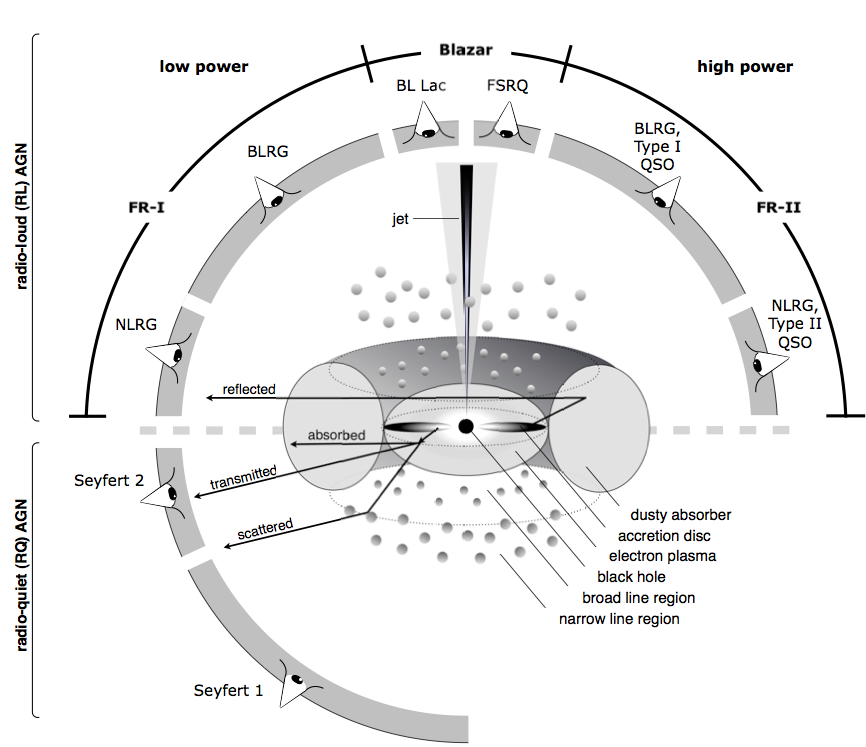
\includegraphics[width=0.7\textwidth]{images/AGNmodel.png} 
\caption[]{Scheme of the unified model of AGN from \citet{Beckmann12}. }
\label{fig:unified_model}
\end{figure}

Fig.\,\ref{fig:unified_model} is a good representation of the unified model of AGN.
The principal component of the engine is a \textbf{supermassive black hole} (SMBH) accreting matter from its surroundings.
The accreting matter is orbiting in an \textbf{accretion disk} and it loses energy, getting close to the SMBH.
The accretion disk has often been accredited as the source of the thermal emission known as the \emph{big blue bump} \citep[e.g.][]{Shang05}.
The SMBH and the accretion disk are surrounded by the so-called \textbf{corona}, a region filled with an electron plasma emitting X-rays via inverse Compton scattering of the photons produced closer to the SMBH \citep{Haardt91}.
Just outside the X-ray corona, there is the \textbf{broad-line region} (BLR), a region of highly ionized gas, distributed in clouds orbiting around the SMBH with velocities of the order of thousands $\si{\kms}$. 
The density of these clouds is relatively high, as it is possible to infer by the absence of broad forbidden lines in optical spectra (see Sec.\,\ref{sec:forb_line}).
All these different structures compose the inner part of an AGN, which is contained within a radius of $\sim 1\,\si{pc}$ from the black hole \citep{Beckmann12}.
In some AGN, a \textbf{relativistic jet} is launched in the region very close to the SMBH. 
The launching mechanism is still far to be fully understood, but the most accredited model to explain this process comes from \citet{Blandford77}, which says that the jet is launched by a strong magnetic field extracting energy from the rotation of the black hole itself.

This inner structure is enclosed in a region of dust rich gas, the \textbf{torus}, which is able to absorb almost all the soft X, ultraviolet, optical and near infrared incident radiation.
Outside the torus, there is another region of ionized gas.
Since it is more distant from the AGN with respect to the BLR, the gas clouds are characterized by a smaller rotational velocity and therefore they emit narrow lines (FWHM $\lesssim 1000\,\si{\kms}$).
Moreover, the electron density is much lower and the gas is able to emit forbidden lines.
This region is known by the name \textbf{narrow-line region} (NLR).

The dimension of the NLR varies in each object, but it is usually between $100\,\si{pc}$ and $1\,\si{kpc}$ \citep{Beckmann12}.
However, in some objects, it is possible to trace the strong emission lines typical of the NLR up to distances of the order of several kiloparsecs.
In some exceptional cases, such as NGC 5252 \citep{Tadhunter89}, Mrk 783 (Sec.\,\ref{cap:paper3}), UGC 7342, NGC 5972 \citep{Keel12} and in another handful of objects, the size of this emission line region can be larger than $20\,\si{kpc}$.
When the size of the NLR is larger than $1\,\si{kpc}$, the structure is often called \textbf{extended narrow-line region} (ENLR) or \textbf{extended emission line region} (EELR).

Among all the described components, the two most important structures needed to explain the AGN properties are the jet and the dusty torus.
The jet is the main driver of radio emission in AGN and its presence should determine if an object is radio-loud or radio-quiet.
The dusty torus instead, is what causes the difference in the optical spectrum of the sources.
The dust in the gas clouds composing the torus is able to completely hide the central part of the AGN to the observer located at high viewing angle with respect to the torus axis.
In this situation, the BLR is not visible and the optical spectrum will be characterized only by the presence of the narrow lines produced in the NLR.
AGN with this property are called Type 2 objects.
Some example of this category of sources are Seyfert 2 galaxies, Narrow-line radio galaxies and Type 2 quasars.
On the other hand, if the angle between the torus axis and the line of sight is small, the observer is able to see the innermost region of the structure.
The BLR is directly visible from the observer and the permitted lines of the spectra show the broad component.
Those sources are called Type 1 AGN and some examples are: Seyfert 1 galaxies, Broad-line radio galaxies, Type 1 quasars.
At very small viewing angle, if a jet is present, the objects appear as blazars (see Fig.\,\ref{fig:unified_model}).
The effects of orientation are observed not only in the optical spectrum but also in other bands of the electromagnetic spectrum, in particular the X-ray spectrum of an obscured (Type 2) and of an unobscured (Type 1) AGN are significantly different, and, for such reason, X-ray surveys have been used to detect and classify AGN. 


\section{The extended narrow-line region}
\label{sec:ENLR}

\begin{figure}
\centering
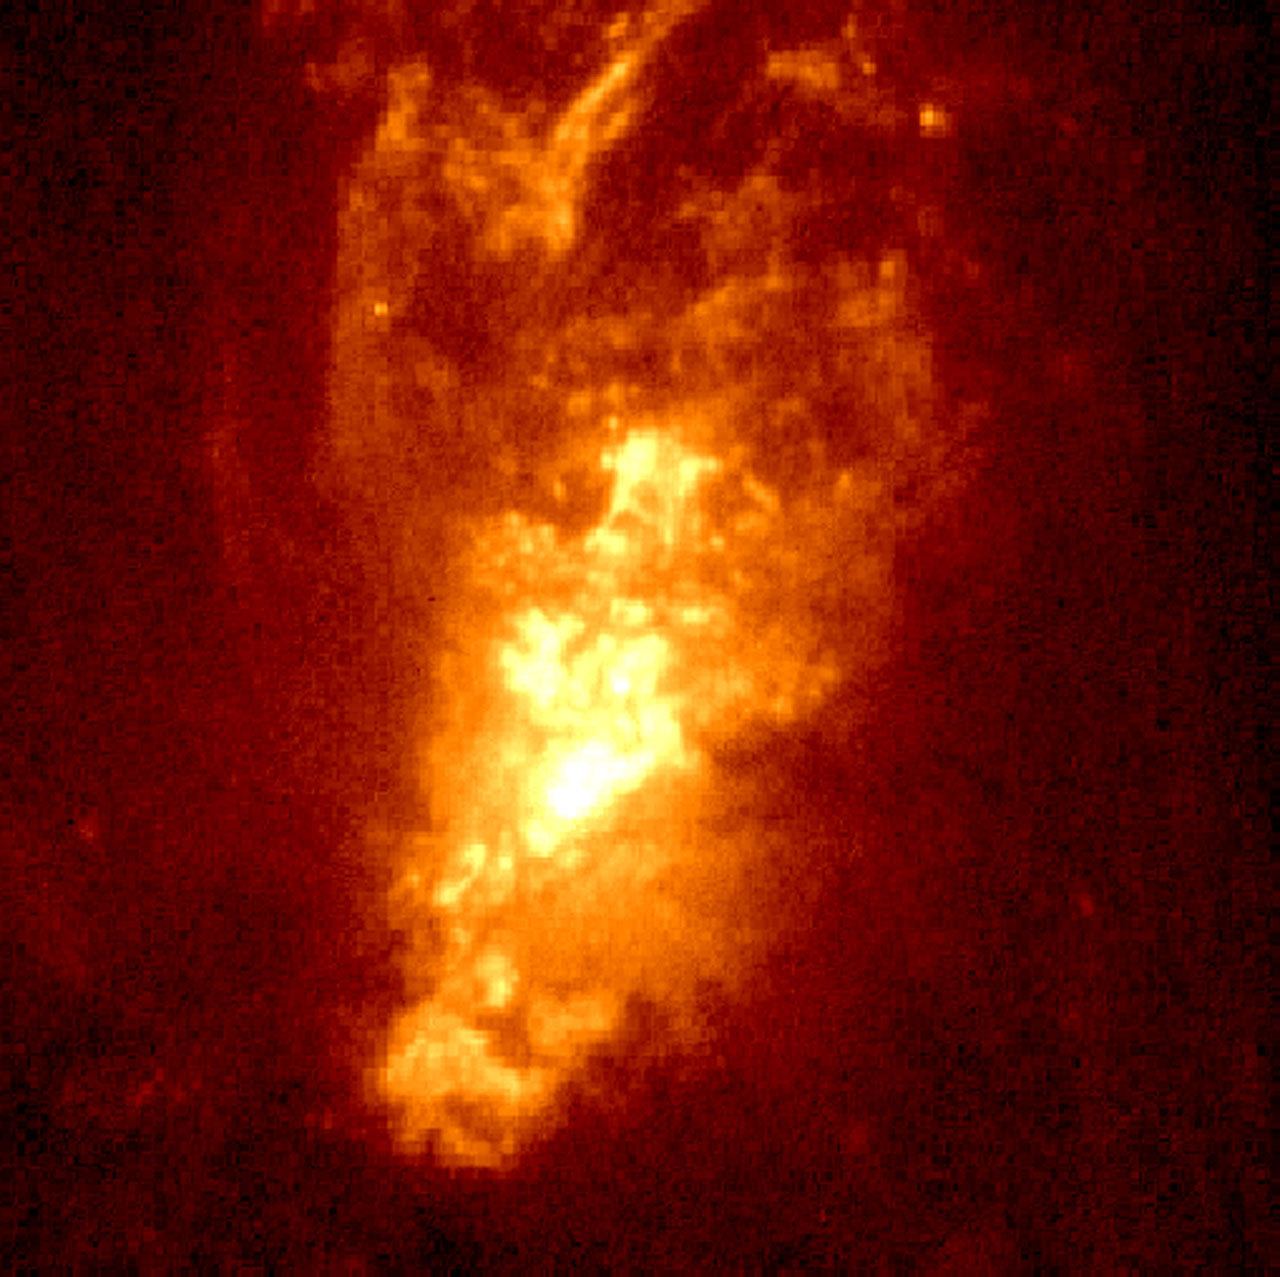
\includegraphics[width=0.7\textwidth]{./images/opo9407c.jpg} 
\caption[]{UV image of the ENLR of the famous Seyfert 2 galaxy NGC 1068. The image has been acquired with the Faint Object Camera (FOC) of the Hubble Space Telescope (HST). The image has been recovered from \url{https://www.spacetelescope.org/images/opo9407c/}}
\label{fig:NGC1068}
\end{figure}

The ENLR is a region of ionized gas that can be considered as a natural prosecution of the NLR when it reaches dimensions that overcome $\sim 1\,\si{kpc}$ (Fig.\,\ref{fig:NGC1068}).
The main difference between the NLR and the ENLR is the observing frequencies of these structures.
The NLR is observed in all AGN with emission lines, while the ENLR is observed only in a handful of objects, $\sim50$ of which are well studied and characterized at $z\le0.05$.
Fortunately, the advent of new integral field spectrographs and relative surveys \citep[e.g. MaNGA,][]{Bundy15} are giving a new pulse to the research and study of these structures \citep{Husemann14,He18}.
The reason for this discrepancy might be a mix of observational biases (e.g. low surface brightness structures need long exposure times with large telescopes) and intrinsic reasons (e.g. gas distribution orientation of the AGN, etc.).
Actually, in the sample described by \citet{Mulchaey96a}, a solid $79\%$ of the observed galaxies (37 out of 47 objects) show resolved and extended line emission \citep{Mulchaey96b}. 
Almost all of them are larger than $1\,\si{kpc}$ and the unresolved ones are the most distant galaxies of the sample.
This suggests that observational biases might be the principal reason for the low number of known ENLRs, combined with the difficulties in resolving them when the redshift starts to increase. 


\subsection{Spectral properties of the ENLR}

Since the ENLR can be considered the natural prosecution of the NLR at large radii, the two structures are characterized by similar spectral and physical properties.

Their spectra show strong, not variable, narrow permitted and forbidden lines, with velocities of the order of $400$--$500\,\si{\kms}$ \citep{Bennert04}. 
The ENLR lines can be a little narrower with respect to that of the NLR, but usually at distances greater than some kiloparsecs from the active nucleus.
This property has been used by early authors \citep[e.g.][]{Unger87} to distinguish an NLR from an ENLR, even though nowadays this distinction is becoming less and less applied.

Several studies that analyzed both multiwavelength observations and ionization models \citep[e.g.][]{Kraemer00,Kallman01} proved that the gas is mostly photo-ionized by the AGN.
The fact that the ionization is produced by the AGN is proved by the wide range of ionization degrees observed in both the NLR and the ENLR.
It is the result of a strong ultraviolet spectrum, much stronger than the typical continuum emitted by young and hot stars \citep{OsterbrockAGN}.
The temperature of the gas, as measured by the ratio of particular forbidden lines (see Sec.\,\ref{sec:forb_line}), is of the order of $10^4\,\si{K}$, much lower than in case of shock heated gas \citep[$T\sim 5\times10^4$ K][]{OsterbrockAGN}.
The presence of forbidden lines proves that the density is lower with respect to their critical density, and actual measurements show a typical range of $10^2$--$10^4\,\si{cm^{-3}}$.

\subsection{Morphology}

Most ENLR have a typical conical or bi-conical shape (e.g. Fig.\,\ref{fig:NGC1068}), with the apexes of the cones pointing towards the AGN.
This peculiar shape is mostly produced by the distribution of the ionizing light.
The radiation originates in the inner part of the AGN, inside the dusty torus.
Due to dust extinction, the ionizing photons can escape only along the axis of the torus.
Therefore, the radiation is collimated, and it assumes the bi-conical shape that is then observed in the distribution of the ionized gas.
For this reason, the existence of ENLRs has always be considered one of the major proof of the validity of the unified model \citep{Wilson94,Schmitt03b,He18}.

\begin{figure}
\centering
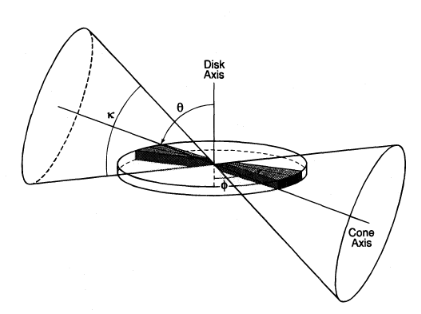
\includegraphics[width=0.7\textwidth]{images/model_diskcone.png} 
\caption[]{Bi-conical ionizing radiation field intersecting a thin disk of gas. The dark area represents the shape of the ENLR in this model. Figure from \citet{Mulchaey96b}.}
\label{fig:disk_model}
\end{figure}

The shape of the ENLR is not determined only by the shape of the ionizing radiation field.
Several other factors actually contribute in the determining its morphology.
The most important one is the distribution of the gas in the host galaxy.
\citet{Mulchaey96b} studied the effects of the gas distribution simulating the morphologies produced by a bi-conical radiation field combined with a spherical or a disk-shaped gas distribution.
The result is that when a disk-shaped distribution produces an ENLR (i.e. the inclination of the cone axis is sufficiently high) the resulting shape is that of a bi-cone (Fig.\,\ref{fig:disk_model}).
This happens both if the line of sight is inside the cone (Type 1 AGN) or outside the cone (Type 2 AGN).

On the hypothesis of a spherical gas distribution, the ENLR is always produced, since the radiation field always intercepts the gas, but the shape changes according to the AGN type.
While Type 2 objects maintain the bi-conical shape, in Type 1 objects the ENLR should assume a halo-like shape.
The comparison of the models with the observations is consistent with a thin disk model for most objects.
But, a consistent number of halo-like ENLR have been observed indiscriminately for Type 1 and Type 2 objects.
This inconsistency is linked mostly to the low spatial resolution of the images which allows confusing small conical ENLR with halo-like ENLR.
In fact, more recent works with higher resolution data \citep[e.g.][]{Schmitt03,Schmitt03b,Fischer13} confirmed that the morphology of the ENLR is consistent with a disk-shaped gas distribution.

However, a property valid in both gas distributions is that the ENLR of Type 1 sources is always smaller with respect to that of Type 2 Sources.
Even though this property has not been confirmed by \citet{Mulchaey96b} comparison of the models with observations, subsequent studies \citep[e.g.][]{Schmitt03b} confirmed that the ENLR of type 1 AGN is smaller, on average, of that of Type 2 sources.

There are exceptions to this rule.
Several Type 1 objects \citep[e.g. NGC 4151][]{Pogge89,Evans93} show large and bi-conical ENLR.
The collimation by a disk-like BLR has been proposed by \citet{Evans93} to explain these exceptions.

An interesting property of the ENLR gas that has been shown by high spatial resolution images of several ENLRs is that the gas is concentrated in clouds, clumps and filaments \citep[e.g.][]{Tadhunter89,Mulchaey96a,Mulchaey96b,Schmitt03,Schmitt03b}, instead of being smoothly and continuously distributed.

\subsection{The origin of the gas}

Up until now, the ionized gas forming the ENLR has always be considered as the gas of the host galaxy disk.
While in some cases this might be true \citep[e.g.][]{Fischer17}, there are several authors that hypothesize other origins for the ENLR gas.
AGN are often characterized by the presence of fast outflows of gas in several different phases, from the cold molecular one to the warm ionized gas \citep{Baldwin87,Hutchings98,Crenshaw00,Crenshaw00b,Dasyra15,Morganti15,Morganti18}.
These outflows usually have a bi-conical shape \citep{Pogge88,Schmitt94,Fischer13} and they might be able to move gas from the nuclear regions to external regions of a galaxy, producing the ENLR.

Another interesting possibility is that the gas is brought in the host galaxy through episodes of merging \citep{Veilleux99,Ciroi05,DiMille07,Cracco11}.
It is now widely accepted that when a galaxy merges with a gas rich companion the newly accreted gas is able to trigger the active phase in the nucleus of the main galaxy \citep{Sanders88,Hong15}.
However, not all the gas involved in the merging arrives in the nucleus but most of it is redistributed in the galaxy and it can be ionized by the AGN radiation producing the ENLR.
This process can be the cause of the presence of ENLR also in early-type galaxies where the gas is expected to be almost absent or in directions not corresponding to that of the galactic disk.

It is not easy to investigate the origin of the ENLR gas.
The spectrum of the ENLR is often characterized by emission lines with disturbed profiles.
Multiple peaks, asymmetries and bumps observed in high-resolution spectra \citep{Ozaki09,Morganti07,Congiu17} are evidence of a disturbed kinematics of the gas, which can be produced by each one of the previously mentioned mechanisms with the addition of the interaction of the interstellar medium (ISM) with the AGN jets.
However, several authors \citep[e.g.][]{Unger87,Fischer17,Fischer18} noticed that, usually, only the inner kiloparsec of the ENLR seems to be perturbed while the remaining part has a kinematics that can be attributed to that of the galaxy disk.
These properties are compatible with the ENLR being mostly composed by the gas of the galactic disk ionized by the AGN while the inner kiloparsecs is disturbed either by gas outflows or by a jet which is expanding in the dense ISM of the galaxy nucleus.



\section{Kiloparsec scale radio emission region}
\label{sec:ksr}

Models suggest that the clouds of the ENLR are accelerated via radiation or wind pressure \citep{Crenshaw00,Crenshaw00b}.
But there are several proofs that the ENLR is aligned with radio structures, i.e. jets, suggesting that there might be a correlation between the ionized gas and the relativistic plasma \citep[e.g.][]{Unger87,Wilson94,Falcke98,Schmitt03,Schmitt03b,Morganti07,Husemann13}.
In particular, jets might expand in the ISM clearing the path for the radiation.
This will make it easier for the radiation to escape from the NLR and to reach more distant gas \citep{Wilson94}.
During this process, the jets interact with the ISM producing shocks and turbulent motion of the gas \citep[e.g.][]{Cracco11,Contini13,Congiu17}.
I will now describe the principal properties of the radio extended emission in AGN, focusing in particular on the so-called kiloparsec scale radio emission region (KSR).
Then I will describe the relationship between the KSR and the ENLR.

\subsection{Principal properties}
\label{sec:princ_prop}

Radio emission is not uncommon in AGN.
\citet{Kellermann16} estimated from $5\,\si{GHz}$ observation of low redshift ($0.2<z<0.3$) quasi-stellar objects (QSO), that almost $20\%$ of them can be considered radio-loud (RL), while the other are considered radio-quiet(RQ).
In particular, \citet{Kellermann16} classified these objects considering RL all the sources with $L_{5_GHz}>10^{23}\,\si{W.Hz^{-1}}$, even though the usual classification is based on the ratio between the flux density at $5\,\si{GHz}$ and in the optical B-band $R=\frac{S_{5\,\si{GHz}}}{F_{B}}$ \citep{Kellermann89}.
According to this classical classification a source is considered RL if $R>10$.

\begin{figure}
\centering
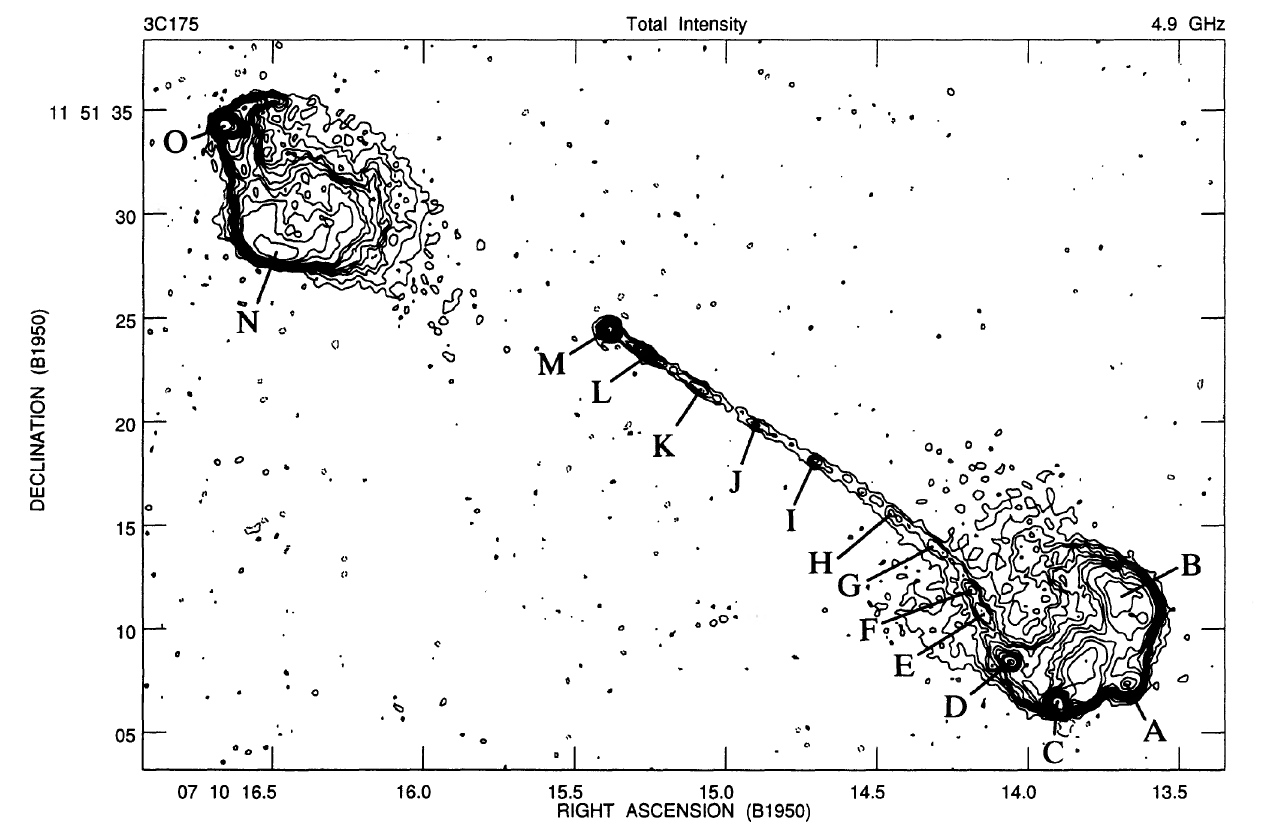
\includegraphics[width=0.7\textwidth]{images/3c175.png} \\
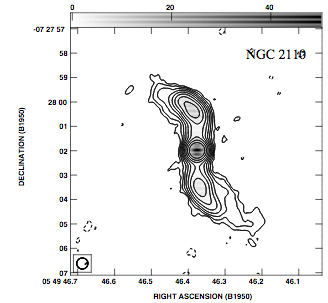
\includegraphics[width=0.7\textwidth]{images/NGC2110.png}
\caption[]{\textbf{Top:} VLA $5\,\si{GHz}$ map of the radio galaxy 3C 175 from \citet{Bridle94}. It is possible to observe both the collimated jet emission and the terminal radio lobes. The extension of the source is $> 300\,\si{kpc}$ \textbf{Bottom:} VLA $1.4\,\si{GHz}$ map of NGC 2110 from \citet{Mundell09}. The maximum extension of this source is $\sim 1\,\si{kpc}$. }
\label{fig:radio_galaxies}
\end{figure}

However, the therm \emph{radio-quiet} does not mean a complete absence of radio emission.
Almost all AGN emit at radio wavelengths, but the sensitivity of modern instruments is not enough to observe the emission in some RQ sources \citep{Kellermann16}.
Nevertheless, it must be pointed out that the emission of RQ seems to be often related to star formation processes happening in the host galaxy, more than to the AGN itself.

RL quasars often show extended bipolar structures (Fig.\,\ref{fig:radio_galaxies}, top panel).
They are caused by relativistic jets launched by the AGN and they can terminate in radio lobes whose extension can surpass hundreds of kpc \citep[e.g][]{Fanaroff74,Perley79,Bridle94}.
On the other hand, RQ-AGN, such as Seyfert galaxies and LINERs usually show compact nuclear emission \citep{Singh15}.
Only occasionally, RQ-AGN show extended radio emission, whose dimension is usually smaller than $\sim 10\,\si{kpc}$ (Fig.\,\ref{fig:radio_galaxies}, bottom panel).
As it has been already introduced, most of the extended emission in RQ-AGN seems to be produced by star formation \citep{Baum93, Kellermann16}.
However, several of them show resolved morphologies similar to jets \citep{Baum93,Colbert96,Morganti99,Gallimore06,Singh15, Singh15b}.
Detailed studies of single objects revealed that Seyfert galaxies, probably the most common class of nearby RQ AGN, are characterized by a morphology of the radio emission consisting in a bright core and one or two jets with relative lobes.
The morphology, therefore, is very similar to the structures observed in RL-AGN, but on much smaller scales (parsec scales vs kiloparsec or megaparsec) \citep[e.g.][]{Wrobel84,Ulvestad87,Morganti99,Kukula99,Momjian03,Kharb06}.

The origin of extended radio emission both in RL and RQ-AGN (when it is not produced by star formation) is related to the presence of jets.
However, we just saw that there is a huge difference between the extension of radio structures in the two classes of objects.
A possible reason for this difference seems related to the properties of the ISM of the objects \citep{Whittle04,Gallimore06,Schawinski11,Singh15b}.
RL AGN with huge extended radio emission are usually found in gas-poor early-type galaxies.
In this case, the jet does not need to dig its way out of the galaxy in a dense ISM.
As a consequence, it preserves most of its energy and it can expand up to several hundred kpc or more.
On the other hand, RQ-AGN seem to be located in gas-rich late-type galaxies.
Their jets seem to be distorted by their interaction with a much denser ISM, which makes them lose more energy and stopping their expansion at much shorter scales.

\subsection{KSR and ENLR}

\begin{figure}
\centering
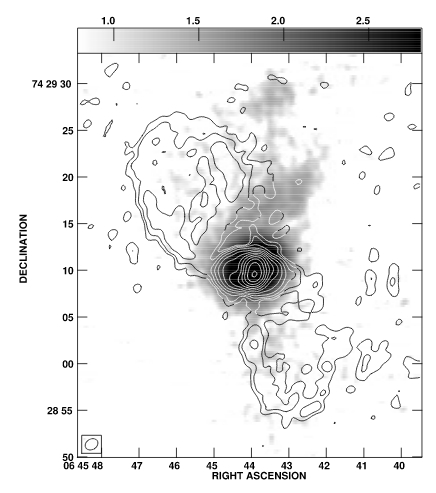
\includegraphics[width=0.7\textwidth]{images/Mrk6_kharb.jpg} 
\caption[]{VLA $5\,\si{GHz}$ contours of Mrk 6 superimposed to an HST [\ion{O}{III}] image of the same source from \citet{Kharb06}. }
\label{fig:mrk6_kharb}
\end{figure}

As it has already been mentioned, several works found that the position angle (PA) of the ENLR is often aligned with the PA of the KSR \citep[e.g.][]{Unger87,Wilson94,Capetti96,Falcke98,Schmitt03,Schmitt03b,Morganti07,Husemann13} (Fig.\,\ref{fig:mrk6_kharb}). 
This happens for most ENLR known so far, therefore there must some kind of connection between the two extended structures.
Just after the first observations of these structures, \citet{Wilson94} hypothesized that the morphology and position of the ENLR must have been a consequence of the action of the jet plasma.
When the jet expands into the ISM it creates a path for the ionizing radiation, produced in the inner part of the AGN, to reach more distant gas with respect to that of the NLR.
This hypothesis has been confirmed a few years later by \citet{Capetti96} who found, for a small sample of Seyfert galaxies, a perfect correspondence between the position and the morphology of the optical and radio extended emission.
For example, in their sample, the presence of radio lobe is always coupled with the shell-like emission line structures, while linear jet radio structures like in Mrk 3 are accompanied by similar morphologies of the ENLR.

Also, the kinematics of the ENLR might be the consequence of the interaction between the jet and the ionized gas.
When the jet pushes the ISM, it creates shocks which can
cause turbulent motion in the gas clouds, heat it and contribute to its ionization \citep[e.g.][]{Steffen97,Morse98,Rodriguez05,Contini12,Congiu17} (Fig.\,\ref{fig:interaction}).

\begin{figure}
\centering
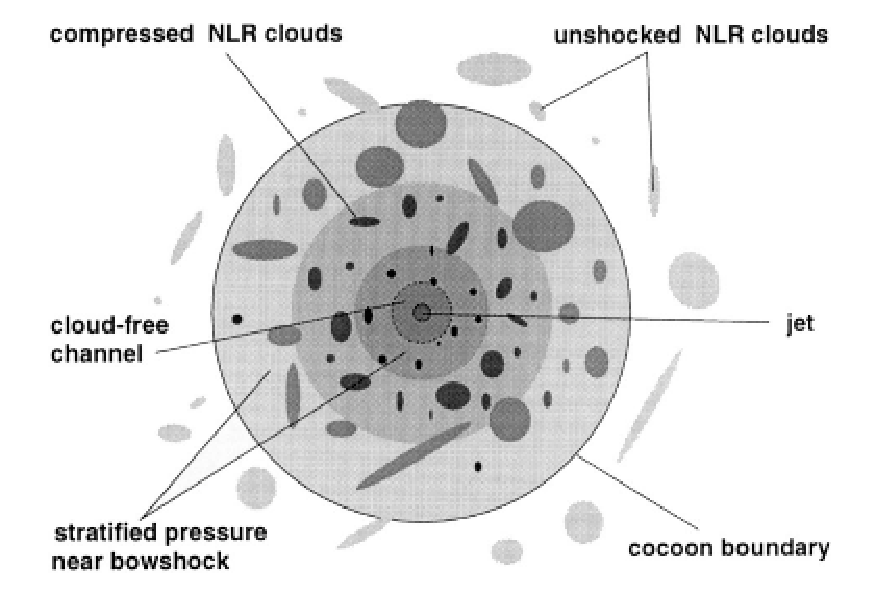
\includegraphics[width=0.7\textwidth]{images/Jet-ism.pdf} 
\caption[]{Scheme from \citet{Steffen97} illustrating the interaction between the jet and the ISM of the NLR.}
\label{fig:interaction}
\end{figure}

The totality of the process through which the AGN interacts with its host galaxy is called AGN feedback.
AGN feedback is usually divided in two types, according to the effect on star formation.
It is considered positive when it produces an enhancement of the star formation, while it is negative when the result is a hampering of this process.
This interplay between the AGN and the host galaxy can happen in two ways: via the interaction of the interstellar medium radiation pressure and wind, the so-called radiative mode, or via interaction between its jets and the ISM, the so-called kinetic mode.
\citet{Fabian12} published a complete review of this argument.

The ENLR is the perfect place to study AGN feedback since both feedback mode can be active in this region.
The main ionizing mechanism of the gas is photo-ionization by the AGN continuum, which can also influence the gas kinematics via radiation pressure (radiative feedback).
On the other hand, the presence of jets interacting with the ISM is the driver of the kinetic feedback.
Therefore, investigating the properties of the gas of the ENLR can help to shed light on this still poorly known processes.



























\biblio
\end{document}